\section{Experiments}\label{sec:experiments}

\begin{figure}
    \centering
    \begin{subfigure}{.3\textwidth}
        \centering
        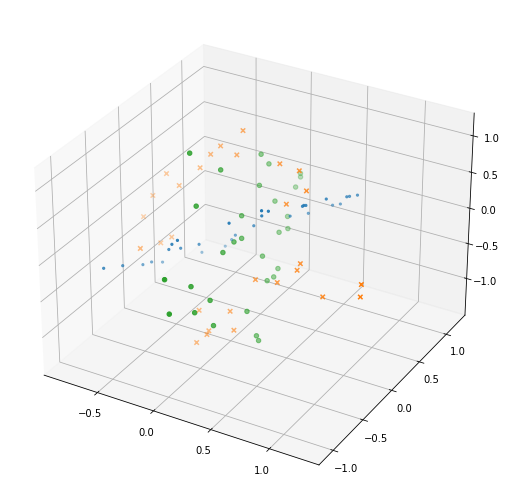
\includegraphics[width=\textwidth]{pics/ds0.png}
        \caption{Dataset 0, $3\times 30$ points.}
    \end{subfigure}%
    \hspace{1em}
    \begin{subfigure}{.3\textwidth}
        \centering
        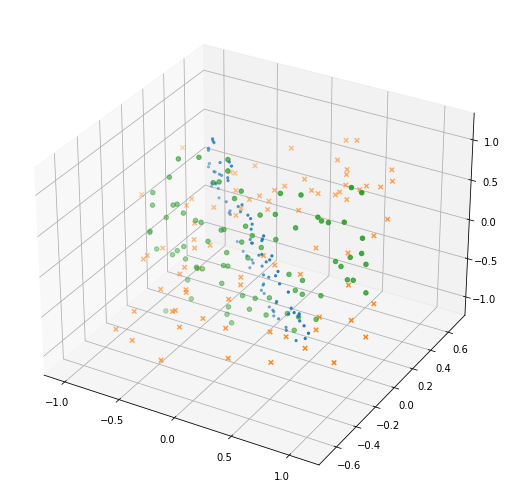
\includegraphics[width=\textwidth]{pics/ds1.png}
        \caption{Dataset 1, $3\times 80$ points.}
    \end{subfigure}%
    \hspace{1em}
    \begin{subfigure}{.3\textwidth}
        \centering
        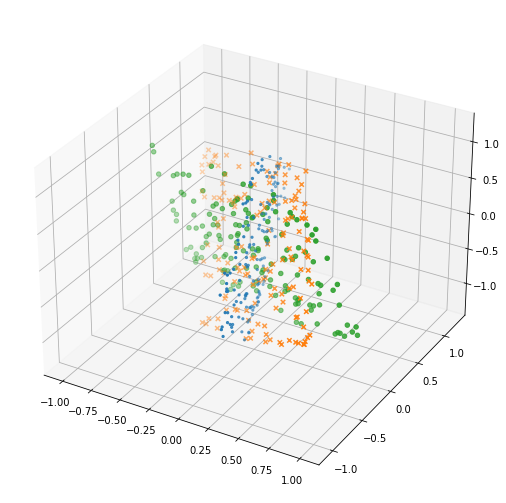
\includegraphics[width=\textwidth]{pics/ds2.png}
        \caption{Dataset 2, $3\times 150$ points.}
    \end{subfigure}%
    \hspace{1em}
    \begin{subfigure}{.3\textwidth}
        \centering
        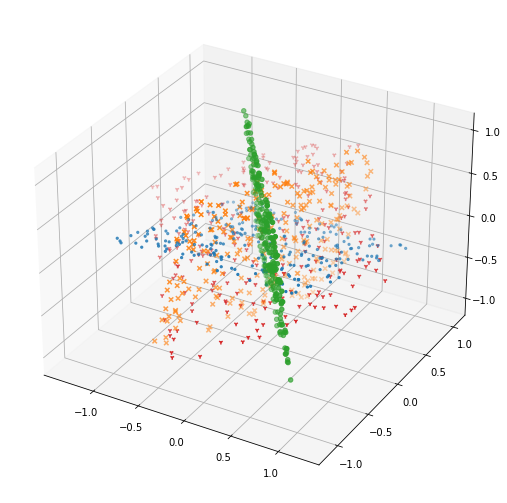
\includegraphics[width=\textwidth]{pics/ds3.png}
        \caption{Dataset 3, $4 \times 250$ points.}
    \end{subfigure}%
    \hspace{1em}
    \begin{subfigure}{.3\textwidth}
        \centering
        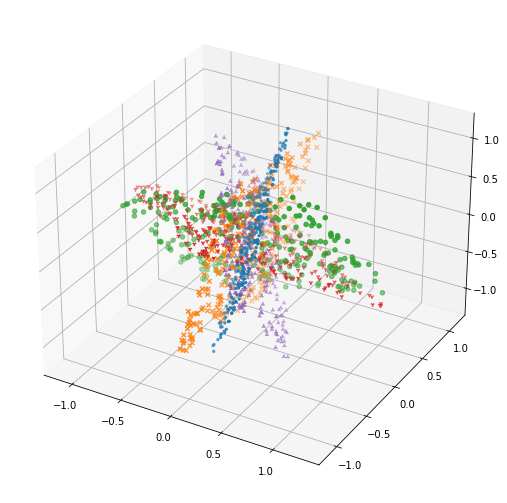
\includegraphics[width=\textwidth]{pics/ds4.png}
        \caption{Dataset 4, $5 \times 300$ points.}
    \end{subfigure}
    \captionsetup{width=.9\linewidth}
    \caption{Generated datasets. Every set contains a number of planes with an equal amount of points. Noise level is $\epsilon = 0.01$.} \label{fig:data}
\end{figure}

We evaluate the proposed algorithms on the following scenario: a collection of 3d-points $P = \{ p_1,\dots,p_s \} \subseteq \R^3$ is sampled from a number of $t$ planes which contain the coordinate origin. We wish to partition the resulting point cloud in such a way that makes the underlying set of planes obvious: i.e., all points that were sampled from a given plane are part of the same set in the partition, distinct from the sets of the other planes. The points are generated as follows. First, every plane is defined by a normal vector and an orientation, i.e. we have vectors $\vec{n}_1,\dots,\vec{n}_t \in \R^3$ and orientations $\vec{o}_1,\dots,\vec{o}_t \in \R^3$. For each plane, we draw $\lambda_i,\lambda_i'$ from $\mathcal{U}([-\pi,\pi))$, and $x_i,x_i'$ from $\mathcal{U}([0,1))$ and determine $\varphi_i = \arccos(2x_i-1), \varphi_i' = \arccos(2x_i'-1)$\footnote{Source: Jason Davies, \href{https://www.jasondavies.com/maps/random-points/}{https://www.jasondavies.com/maps/random-points/}. Accessed on December 6th, 2020.}. The vectors are computed by $$ \vec{n}_i = \begin{bmatrix} \sin(\varphi_i) \cos(\lambda_i) \\ \sin(\varphi_i)\sin(\lambda_i) \\ \cos(\varphi_i) \end{bmatrix},\quad \vec{o}_i = \mathrm{norm} \left( \begin{bmatrix} \sin(\varphi_i') \cos(\lambda_i') \\ \sin(\varphi_i')\sin(\lambda_i') \\ \cos(\varphi_i') \end{bmatrix} \times \vec{n}_i \right), $$ where $\mathrm{norm}(\vec{h})=\vec{h} / ||\vec{h}||  $ ($\vec{n}_i$ has already normalized length, since it describes a point on the unit-sphere). Secondly, for every point $p_i$, three components are sampled: the 2d-position on the plane $x_i,y_i$ from $\mathcal{U}([-1,1])$, and a noise-component $z_i$ from $\mathcal{U}([-\epsilon,\epsilon])$ (where $\epsilon$ indicates the level of noise). The point is then transformed into plane-space, i.e. $$ p_i = x_i \vec{o}_i + y_i \mathrm{norm}(\vec{o}_i \times \vec{n}_i) + z_i \vec{n}_i.$$
For three points $u,v,w \in P$, we define the following cost-structure
\begin{align*}
    c(\{u,v,w\}) &= 0, \\ 
    \quad c'(\{u,v,w\}) &= \mathrm{d}(\{ u,v,w \},(0,0,0)) - \tau, \\
    \mathrm{d}(\{u,v,w\},p) &= \frac{\vec{n} \cdot (u - p)}{||\vec{n}||},\quad \vec{n} = (v-u)\times (w-u),
\end{align*}
where $\mathrm{d}(\{u,v,w\},p)$ is the distance between the plane that contains $u,v$ and $w$ and $p$ (``$\cdot$'' is the dot-product in this case) and $\tau$ is some small value. Therefore, if the distance from the plane spanning over $u,v$ and $w$ to the origin ist smaller than $\tau$, it is considered ``good'' when $u,v$ and $w$ are part of the same set and if the distance is large, it is considered ``bad''.

\begin{table}[ht]
    \centering
    \captionsetup{width=.9\linewidth}
    \begin{tabular}{l|llll|lll}
        run & dataset & {\bf is} & $N$ & $M$ & {\bf or} [s] & {\bf iter} & {\bf or}/{\bf iter} [s] \\
        \hline 
        0-S-S  & 0 & 1 & 40 &  1000       & 3.24 & 159 & 0.020       \\   
        0-E-S  & 0 & 1 & -- &  1000       & 24.66 & 103 & 0.239      \\   
        0-S-E  & 0 & 1 & 40 &  --         & 5.54 & 191 & 0.029       \\   
        0-E-E  & 0 & 1 & -- &  --         & 18.30 & 68 & 0.269       \\ 
        \hline 
        1-S-S  & 1 & 1 & 40 &  5000       & 16.68 & 439 & 0.038      \\   
        1-E-S  & 1 & 1 & -- &  5000       & 949.42 & 375 & 2.532     \\   
        1-S-E  & 1 & 1 & 40 &  --         & 59.18 & 461 & 0.128      \\   
        1-E-E  & 1 & 1 & -- &  --         & 473.91 & 143 & 3.314     \\   
        \hline
        2-S-S  & 2 & 1 & 50 &  5000       & 47.41 & 988 & 0.048      \\   
        3-S-S  & 3 & 1 & 50 & 10000       & 321.57 & 4532 & 0.071    \\   
        4-S-S  & 4 & 1 & 50 & 15000       & 1078.05 & 10000 & 0.108  \\   
        \hline
        2-S-SL & 2 & 1 & 50 &   500       & 48.06 & 2341 & 0.021     \\   
        2-SL-S & 2 & 1 &  5 &  5000       & 65.49 & 8498 & 0.008     \\   
        \hline
        2-S-S-IP10  & 2 &  10 & 50 & 5000 & 71.68 & 1440 & 0.050     \\   
        2-S-S-IP50  & 2 &  50 & 50 & 5000 & 77.64 & 1556 & 0.050     \\   
        2-S-S-IP100 & 2 & 100 & 50 & 5000 & 101.04 & 2035 & 0.050
    \end{tabular}
    \caption{Every run with the corresponding dataset it was executed on, the number of {\bf i}nitial {\bf s}ets in the partition, the number of neighbours $N$ and samples $M$ that are selected per iteration, the {\bf o}verall {\bf r}untime and number of {\bf iter}ations. If entries for $N$ or $M$ are ``--'', then this means that the complete neighbourhood was considered, or the reduced costs were computed explicitly. For each run, $\tau$ was set to $0.1$ and the stopping criterion was chosen in such a way that the randomized runs take at least 50 iterations and stop when the correct number of sets was reached. The deterministic runs ($N$ and $M$ both ``--'') search until no improving move exists.} \label{tab:runs}
\end{table}
The algorithms are evaluated in the four following settings on the datasets seen in figure \ref{fig:data} (all runs shown in table \ref{tab:runs}). First, the deterministic greedy search is compared with randomized versions, in which only a certain subset of neighbours is selected and/or the reduced cost is only approximated. This is done on the two datasets 0 and 1, in which dataset 0 contains $3 \times 30$ points, and dataset 1 overall $3 \times 80$ points. In the second setting, problems with larger input-sizes are considered and solved by the randomized greedy search algorithm (dataset 2, 3 and 4 with $3 \times 150$, $4 \times 250$ and $5 \times 300$ points respectively). The penultimate setting examines the impact of low neighbourhood- and sampling sizes on the number of iterations. Finally, the randomized greedy search algorithm is initialized with random partitions. The results are shown in figures \ref{fig:setting11}, \ref{fig:setting12}, \ref{fig:setting2}, \ref{fig:setting3} and \ref{fig:setting4}. The upper rows show how much the costs are reduced in each iteration\footnote{If the reduced costs are negative in an iteration, then this means that none of the considered neighbours yields an improvement over the current assignment.}, the middle rows contain the used time per iteration -- the cumulative time to compute the reduced cost for each neighbour in orange, and the time required to compute the neighbourhood in blue -- and the last rows show the number of sets in the partitions per iteration. All runs (except for the runs in setting 4) start with a partition where all vertices have the same set. 
\\
An observation that can be made beforehand with respect to all considered settings is that all instances of the greedy search with sampling tend to increase the number of sets in the partitions in the beginning while decreasing them in the end. This might be caused by the definition of the cost function: if many 3-ary subsets of vertices share the same set in the partition even if they are assigned high costs, it might be better to just split them up. Similarly, if the number of sets in the partitions is high, the probability that a vertex is assigned a set that ``fits'', i.e. yields negative costs, is higher.


\paragraph{Setting 1.} Deterministic and randomized greedy search are compared on datasets 0 and 1, with $3 \times 30$ (runs 0-S-S, 0-E-S, 0-S-E, 0-E-E) and $3 \times 80$ (runs 1-S-S, 1-E-S, 1-S-E, 1-E-E) points respectively. The results are depicted in figures \ref{fig:setting11} and \ref{fig:setting12}. When the complete neighbourhood is considered, as for run 0-E-S, 0-E-E, 1-E-S and 1-E-E, the used time per iteration is clearly dependent on the number of sets in the partitions (figure \ref{fig:setting11}, \ref{fig:setting12} middle row). This is obvious from analysis of algorithm \ref{alg:moveenum}, since the number of neighbours grows in size $O(|V| \cdot |\Pi(\idx)|)$. Considering the complete neighbourhood has probably the largest impact on the overall runtime, as can be seen in table \ref{fig:data}. However, the number of iterations does not increase significantly when decreasing the amount of neighbours (compare 0-S-S with 0-E-S or 1-S-S with 1-E-S), which suggests that the probability of selecting a random neighbour that lowers the costs is relatively high. This would mean that in every iteration, there are multiple ways of selecting a ``good'' neighbour, instead of only one. Computing the reduced costs for every possible pairing of vertices also takes a lot of time, as can be seen in run 1-S-S in comparison to 1-S-E, but also has no meaningful impact on the number of iterations.

\paragraph{Setting 2.} We want to check the performance of the randomized search when considering comparatively larger problem instances, i.e. the partitioning of dataset 2, 3 and 4, see table \ref{fig:data}. Here, the size of the considered neighbourhood for runs 2-S-S, 3-S-S and 4-S-S (figure \ref{fig:setting2}) is set to $N=50$ neighbours, but the number of samples to compute the reduced costs was increased with growing problem size ($5000, 10000$ and $150000$ respectively). The performance of the randomized algorithm stays consistent with respect to every problem instance and yields an almost constant time requirement in each iteration. Only in the beginning there is a slight increase in the used time required to compute the (estimated) reduced costs (figure \ref{fig:setting2}, middle row). This has to do with the definition of the cost-function: if there is only a low number of sets in the partitions, the likelihood of sampling a 3-ary subset that contains vertices which share the same set is high. Since only the computation of $c'$ is expensive (in comparison to $c$), this yields an increased computational load.

\paragraph{Setting 3.} The third setting compares the impact of small neighbourhoods (2-SL-S, $N=5$) and small sample sizes (2-S-SL, $M=500$) on the number of iterations/overall runtime with ``ordinary'' sizes (2-S-S, $N=50, M=5000$). See figure \ref{fig:setting3} for runs 2-SL-S and 2-S-SL and figure \ref{fig:setting2} for 2-S-S. Both for small sample sizes and small neighbourhoods, one can see that the number of iterations increases (figure \ref{fig:setting3}, bottom row). This is expected, since large neighbourhoods and large sample sizes enable precise decision making in each iteration, and therefore lower the overall amount of iterations. However, since computation time per iteration decreases with lower neighbourhood/sample sizes, it may be possible that the overall runtime decreases as well. This is the case for run 2-S-SL, as can be seen in table \ref{fig:data}, but not for run 2-SL-S (although both settings do not decrease/increase the overall runtime significantly). Another observation is that the number of sets in the partitions per iteration yields a different shape for low neighbourhood sizes (run 2-SL-S, bottom row): a stark increase in the beginning with a small gradual decrease afterwards.

\paragraph{Setting 4.} The final setting examines the impact of different initializations on the number of iterations (runtime per iteration should be approximately equal, since $N$ and $M$ are left unchanged -- therefore, the overall runtime should only depend on the number of iterations). Run 2-S-S-IP10 assigns every vertex one of 10 different sets, 2-S-S-IP50 assigns every vertex one of 50 different sets and 2-S-S-IP100 assigns every vertex one of 100 different sets (figure \ref{fig:setting4}). As can be seen from figure \ref{fig:setting4}, the number of iterations increases with growing number of initial assignments. A reason for this might be that the probability that two random vertices have the same set is low if the number of sets in the partitions is high. Since the costs were only defined on vertices sharing the same set, this might decrease the quality of the estimated costs.
\\
Similarly to the previous setting, the number of sets in the partitions per iteration behave differently for the considered runs (figure \ref{fig:setting4}, bottom row). For run 2-S-S-IP10, the curve (growth in the beginning, drop in the end) is similar to that of run 2-S-S. Run 2-S-S-IP50 increases the number of sets in the beginning only slightly, and run 2-S-S-IP100 stays almost constant before dropping to the optimal number.

From the above observations, we are able to draw the following conclusions with respect to the considered scenario. First, if $M$ and $N$ are chosen appropriately, the randomized version outperforms the deterministic version significantly when it comes to overall runtime. Especially the selection of a relatively low neighbourhood size yields a great time advantage, but the importance of selecting $M$ not too high as well grows with more vertices (and planes). Second, the randomized greedy search yields consistent results if the problem size grows and allows for almost constant time requirements per iteration. Third, Selecting $M$ relatively low yields the requirement for a greater number of iterations, but since every iteration is faster, the overall required time might decrease. Same for $N$. And finally, increasing the number of initial sets in the partition yields a greater number of iterations and a worse runtime.


\begin{landscape}
    \begin{figure}
        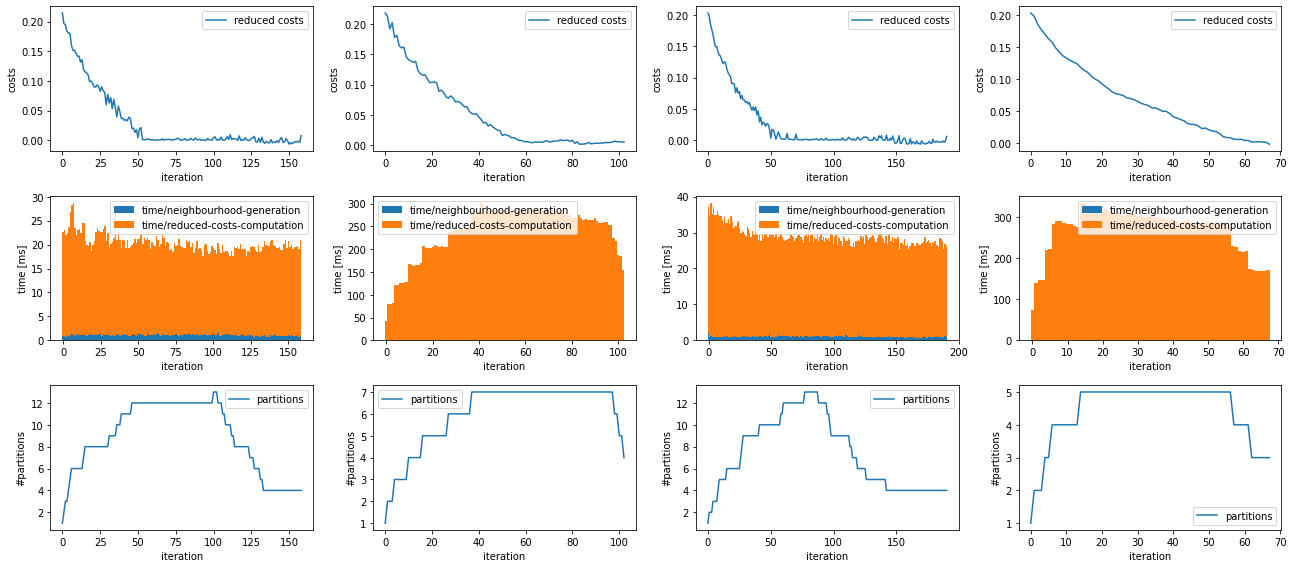
\includegraphics[width=22cm]{pics/experiments_0.png}
        \caption{From left to right: run 0-S-S, 0-E-S, 0-S-E, 0-E-E.}
        \label{fig:setting11}
    \end{figure}
\end{landscape}


\begin{landscape}
    \begin{figure}
        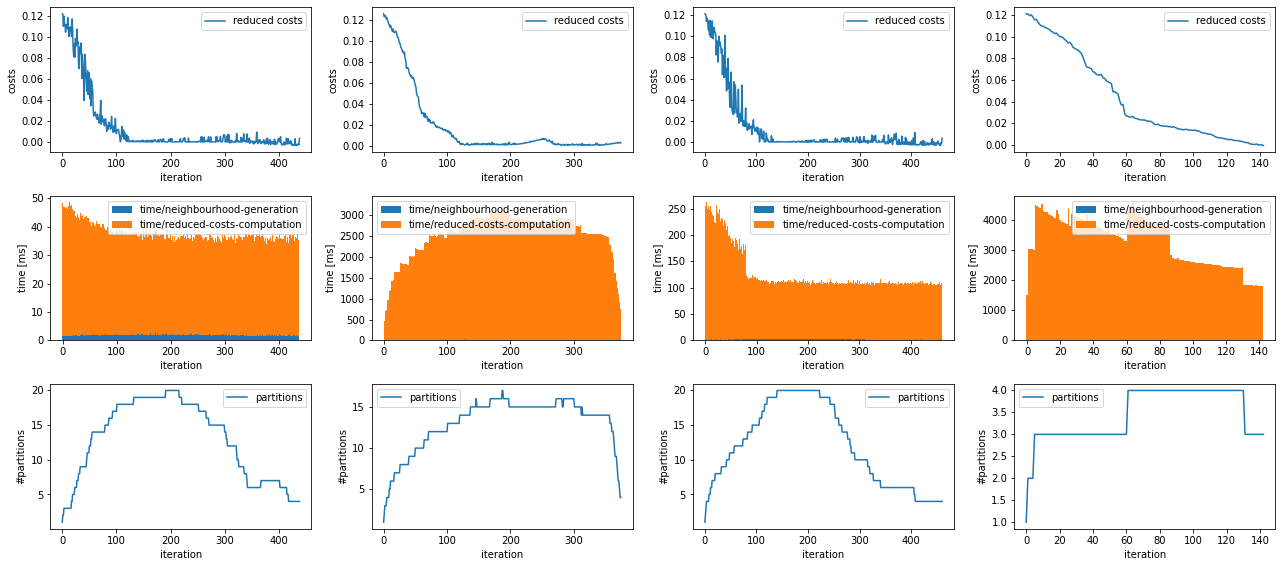
\includegraphics[width=22cm]{pics/experiments_1.png}
        \caption{From left to right: run 1-S-S, 1-E-S, 1-S-E, 1-E-E.}
        \label{fig:setting12}
    \end{figure}
\end{landscape}

\begin{landscape}
    \begin{figure}
        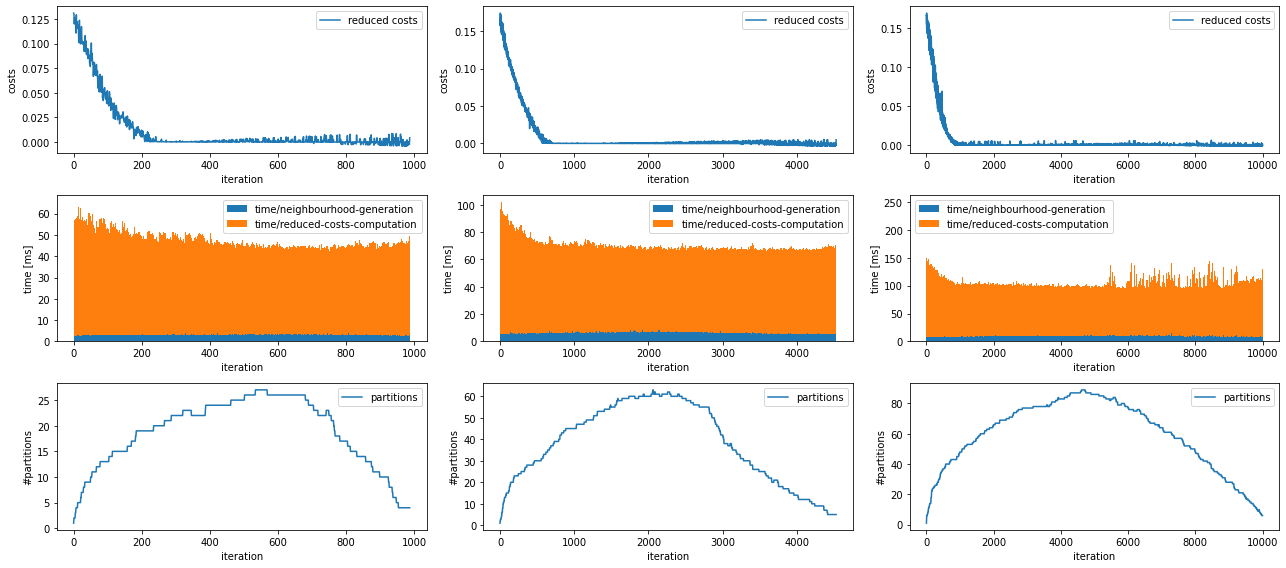
\includegraphics[width=22cm]{pics/experiments_2.png}
        \caption{From left to right: run 2-S-S, 3-S-S, 4-S-S.}
        \label{fig:setting2}
    \end{figure}
\end{landscape}

\begin{landscape}
    \begin{figure}
        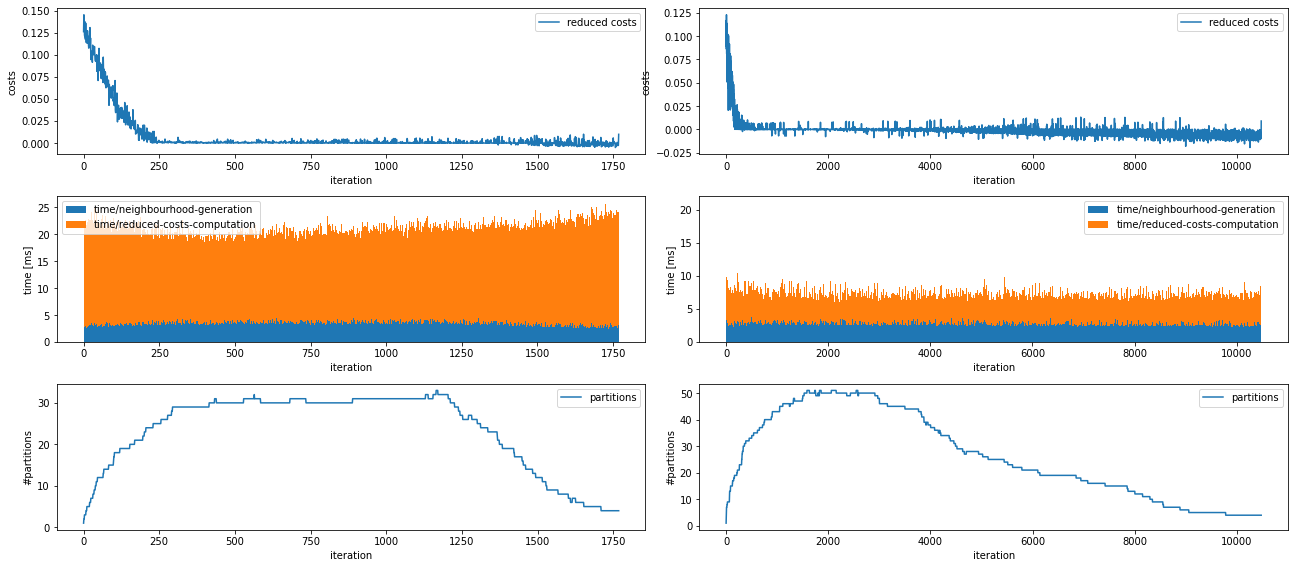
\includegraphics[width=22cm]{pics/experiments_3.png}
        \caption{From left to right: run 2-S-SL, 2-SL-S.}
        \label{fig:setting3}
    \end{figure}
\end{landscape}

\begin{landscape}
    \begin{figure}
        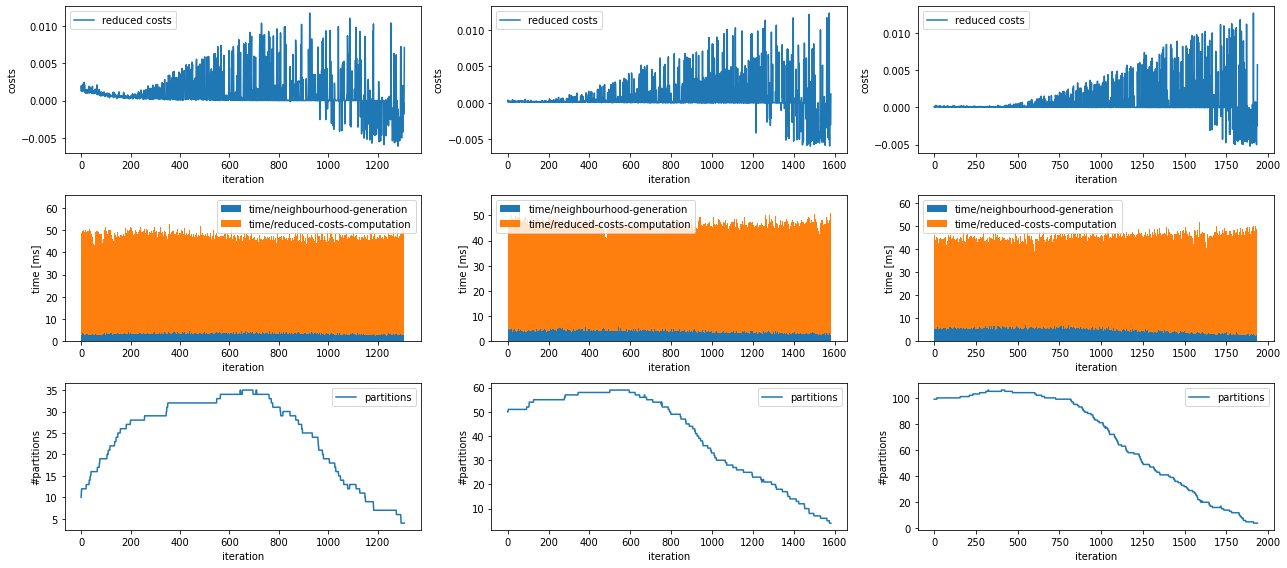
\includegraphics[width=22cm]{pics/experiments_4.png}
        \caption{From left to right: run 2-S-S-IP10, 2-S-S-IP50, 2-S-S-IP100.}
        \label{fig:setting4}
    \end{figure}
\end{landscape}

\section{Conclusion and Possible Improvements}
This project investigated a datastructure and (probabilistic) local-search methods for solving the partitioning-problem with respect to cost functions defined on 3-ary subsets of the given set. A special focus was put on the space- and time-efficiency of the used datastructure and fast improvements in each iteration. For this matter, the neighbourhood of a solution (partition) was defined over the set of possible ``moves'' of one vertex to another set, and an efficient way of enumerating the neighbourhood of a partition was given. In this regard, an algorithm for selecting random neighbours was defined, which allows for a comparatively fast way of sampling neighbours. In the end, the proposed datastructure and sampling-based methods were evaluated on a set of different experiments, which underlined the theoretical results. 
\\
Possible further investigations could include the following points. Using the theoretical results in Theorem \ref{theorem:equal_indexings}, it is possible to check the equality of two partitions induced by indexings in time $O(|V|)$. This could be of use when implementing local search algorithms like Tabu-Search (Glover \cite{glover1986future}) which keep track of previous solutions and require to compute whether new solutions are equal to past ones. On the same note, on could think of a Tabu-Search implementation that keeps track of which vertex was moved in the near past and then only considers neighbours that do not move these respective vertices. Another extension would be the implementation of simulated annealing, in which the fast way of selecting random neighbours might be helpful.

% randomized >> deterministic
% choosing the sample and neighbourhood size optimally
% choose the number of neighbours low in the beginning and high in the end
% in the beginning there are many "good" moves and in the end there are few
% choose the neighbourhood proportional to |V| * | \Pi(\idx) | 
% in this setting: low initial number of partitions is better

% points i want to make:
% sampling neighbours and costs is really efficient when |V| grows larger
% evaluating the neighbourhood and computing the complete costs does not really work for large |V|
% M needs to be choosen sufficiently large, or else it does not converge
% possible improvements: sample only vertices such that the resulting costs is non-zero
% M needs to be somewhat proportional to |V| and the expected variance: i.e., dependent on the 
% number of partitions
% number of planes -> impact on the variance
% do we need 

% possible improvements:
% taboo-search should be efficient to implement:
%   if complete partitions can be "taboo", then the result of theorem.... yield a fast way of
%   comparing different indexing for equality of their induced partitions
%   if only vertices can be taboo, e.g. if they were moved, then keeping a simple n-d array would
%   be sufficient. the neighbourhood-generation would have to be rewritten of course 
% simulated annealing should also be easy -- drawing random neighbour can be done relatively fast
% since the candidate generation can be done fast
